\documentclass{xmgr}

\makeatletter
\newcommand\footnoteref[1]{\protected@xdef\@thefnmark{\ref{#1}}\@footnotemark}
\makeatother

\author   {Daniel Sienkiewicz}
\nralbumu {206358}
\email    {daniel@sienkiewicz.ovh}


\title    {Projekt komputera samochodowego bazujący na systemie mikrokomputera Intel Galileo}
\date     {2015}
\miejsce  {Gdańsk}

\opiekun  {dr inż. Janusz Młodzianowski}

\begin{document}

\begin{abstract}
Celem pracy jest stworzenie komputera pokładowego do samochodu, w którego skład wchodzi: \begin{enumerate}
\item Mikrokomputer Intel Galileo Gen 1, 
\item Ekran dotykowy FTDI VM800, 
\item Oprogramowanie,
\item Kamerka cofania.
\end{enumerate}

Pierwsza część pracy przedstawia architekturę projektu wraz z jego opisem funkcjonalnym. Opisuję również mechanizmy komunikacji systemu mikroprocesorowego z otoczeniem.

Następnie przedstawiony jest pomysł implementacji oraz proces tworzenia niezbędnej do obsługi symulatora samochodu biblioteki pozwalającej na komunikację z I/O Expanderem PCF8574N.

Ostatnia część pracy przedstawia pomysły  możliwych rozszerzeń projektu o dodatkowe moduły oraz funkcjonalności w zależności od potrzeb użytkownika.
\end{abstract}
\keywords{Intel Galileo, $I^2C$,
 SPI, 
 C, 
 Arduino,
 GPIO,
 FTDI Chip,
 VM800}
\maketitle

%================WPROWADZENIE=====================
\chapter{Wprowadzenie}
\section{Cele}
Celem pracy jest budowa oraz oprogramowanie komputera pokładowego do samochodu. Komputer powinien móc wczytać z czujników temperaturę panującą w silniku, na zewnątrz oraz w środku samochodu. Ponadto powinien on móc zapisać aktualną pozycję GPS na karcie microSD oraz umożliwić korzystanie z kamerki cofania lub inteligentnego lusterka wstecznego.
\section{Założenia}
Do wykonania komputera wykorzystano: Intel Galileo używane w trybie Arduino o oprogramowywane za pomocą Arduino IDE, lokalizator GPS służący do podawania aktualnej pozycji dzięki której obliczana zostaje droga przebyta przez samochód, kamerka internetowa służąca jako czujnik cofania oraz inteligentne lusterko wsteczne oraz symulator samochodu. Aktualnie komputer nie będzie zamontowany do fizycznego samochodu więc do tych celów zbudowany został symulator samochodu składający się z podstawowych czujników takich jak: guziki służące za czujnik zapięcia pasów/zamknięcia drzwi, potencjometry służące za czujniki temperatury oraz I/O expander PCF8574N pozwalający zmniejszyć ilość kabli wychodzących z symulatora do Intel Galileo do 2 zamiast 11. Na komputerze nie będzie wyświetlana aktualna prędkość ani przebieg ponieważ nawet w najnowszych samochodach nie jest to dostępna opcja. Dane te są dostępne na zegarach samochodowych więc nie ma potrzeby powtarzania tej informacji.
\section{Plan pracy}
TO DO
%================KONIEC WPROWADZENIE=====================

%================ARCHITEKTURA=====================
\chapter{Architektura}
\subsection{Opis funkcjonalny}
\subsection{Mechanizmy komunikacji systemu mikroprocesorowego z otoczeniem}
\subsubsection{Porty}
TO DO
\subsubsection{Przerwania}
TO DO
\subsubsection{Odpytywanie w pętli}
TO DO
\subsubsection{Timer}
TO DO
\subsubsection{Protokół komunikacyjny}
TO DO
\subsubsection{Złączki oraz kable}
TO DO
\subsection{Intel Galileo}

\begin{figure}[!htb]
    \centering
    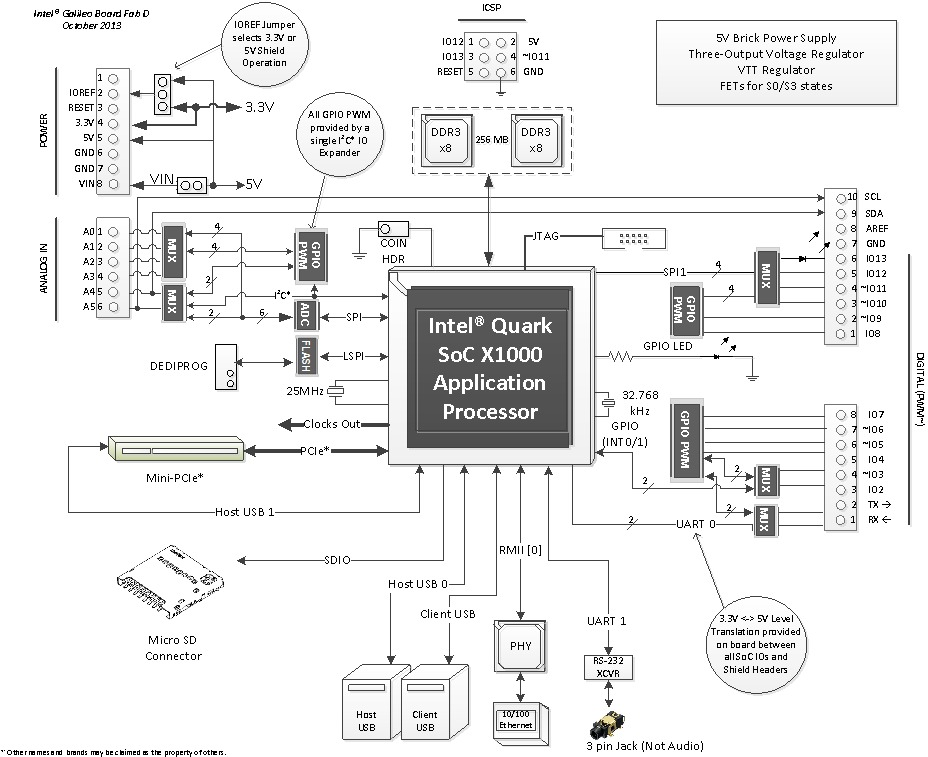
\includegraphics[height=0.3\textheight]{images/IntelGalileoLogicSchematics.jpg}
    \caption{Schemat logiczny układu Intel Galileo\label{IntelGalileoLogicSchematics}}
    \source{\url{https://www.arduino.cc/en/ArduinoCertified/IntelGalileo}}
\end{figure}

%================KONIEC ARCHITEKTURA=====================

%================IMPLEMENTACJA=====================
\chapter{Implementacja}
\section{$I^2C$}
\subsection{Problemy z bibliotekami}
\subsection{moja implenatacja $I^2C$ (read)}
\subsection{Schemat blokowy programu}

\begin{figure}[!htb]
    \centering
    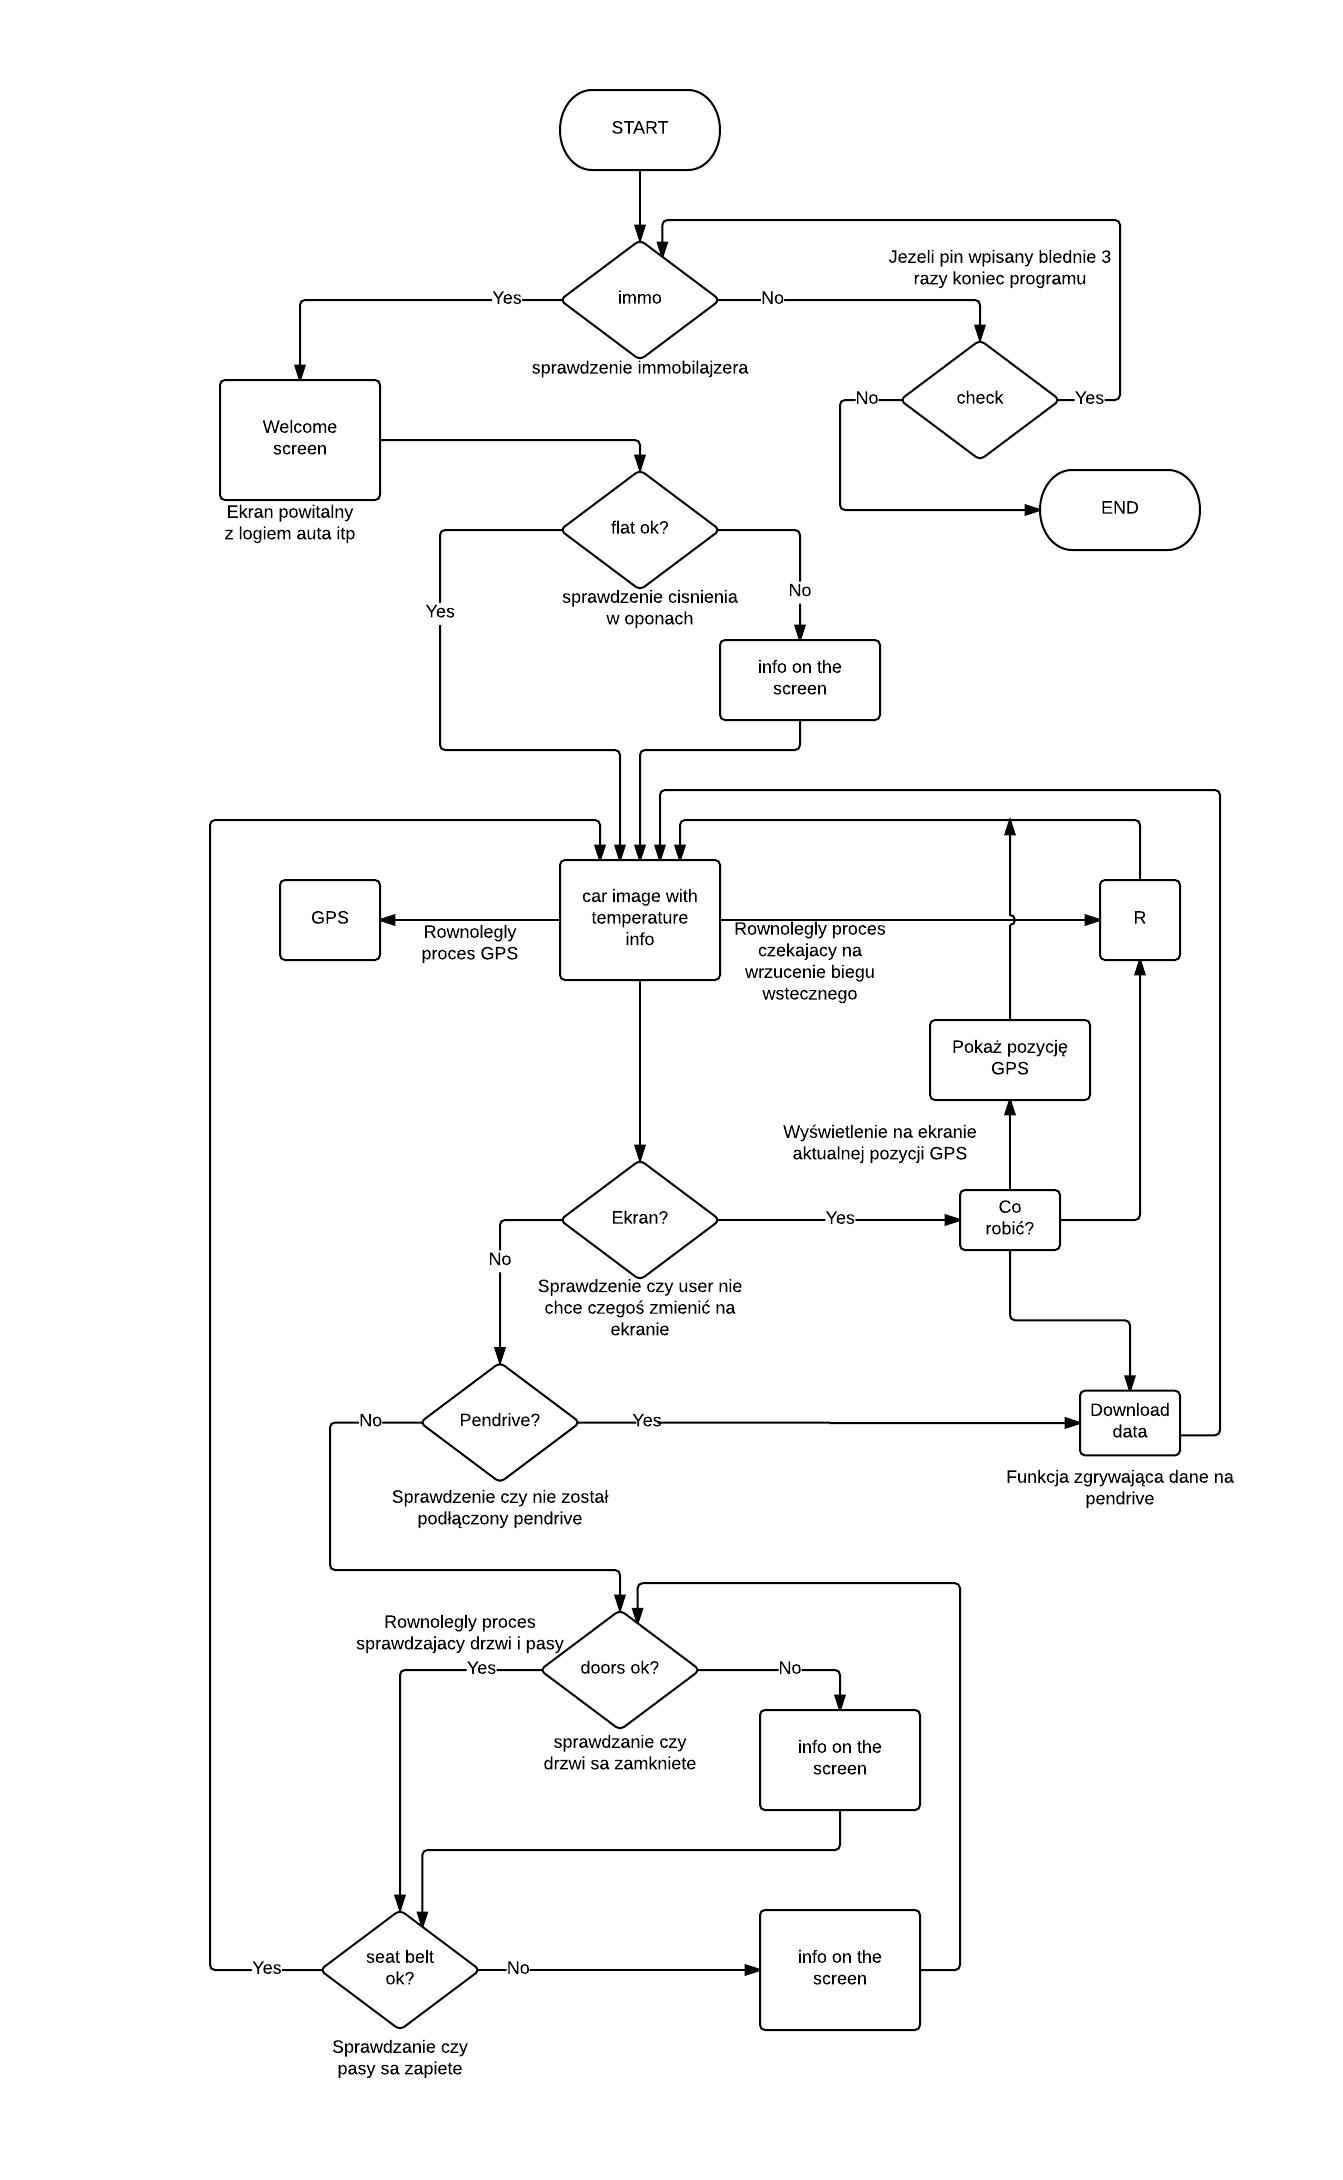
\includegraphics[height=0.4\textheight]{images/schemat_blokowy.png}
    \caption{Schemat blokowy głównego programu\label{SchematBlokowy}}
    \source{Opracowanie własne}
\end{figure}

\subsection{Moja biblioteka do R/W Arduino dla Intel Galileo}
\section{Założenia funkcjonalne}
 - czytanie z czujników, pisanie do ekranu, czytanie z ekranu
 - włączanie i wyłączanie systemu
\section{Integracja z samochodem}
 - podpięcie pod auto
 - włączanie i wyłączanie systemu - można brutalnie wyłączyć
 
 \begin{figure}[!htb]
    \centering
    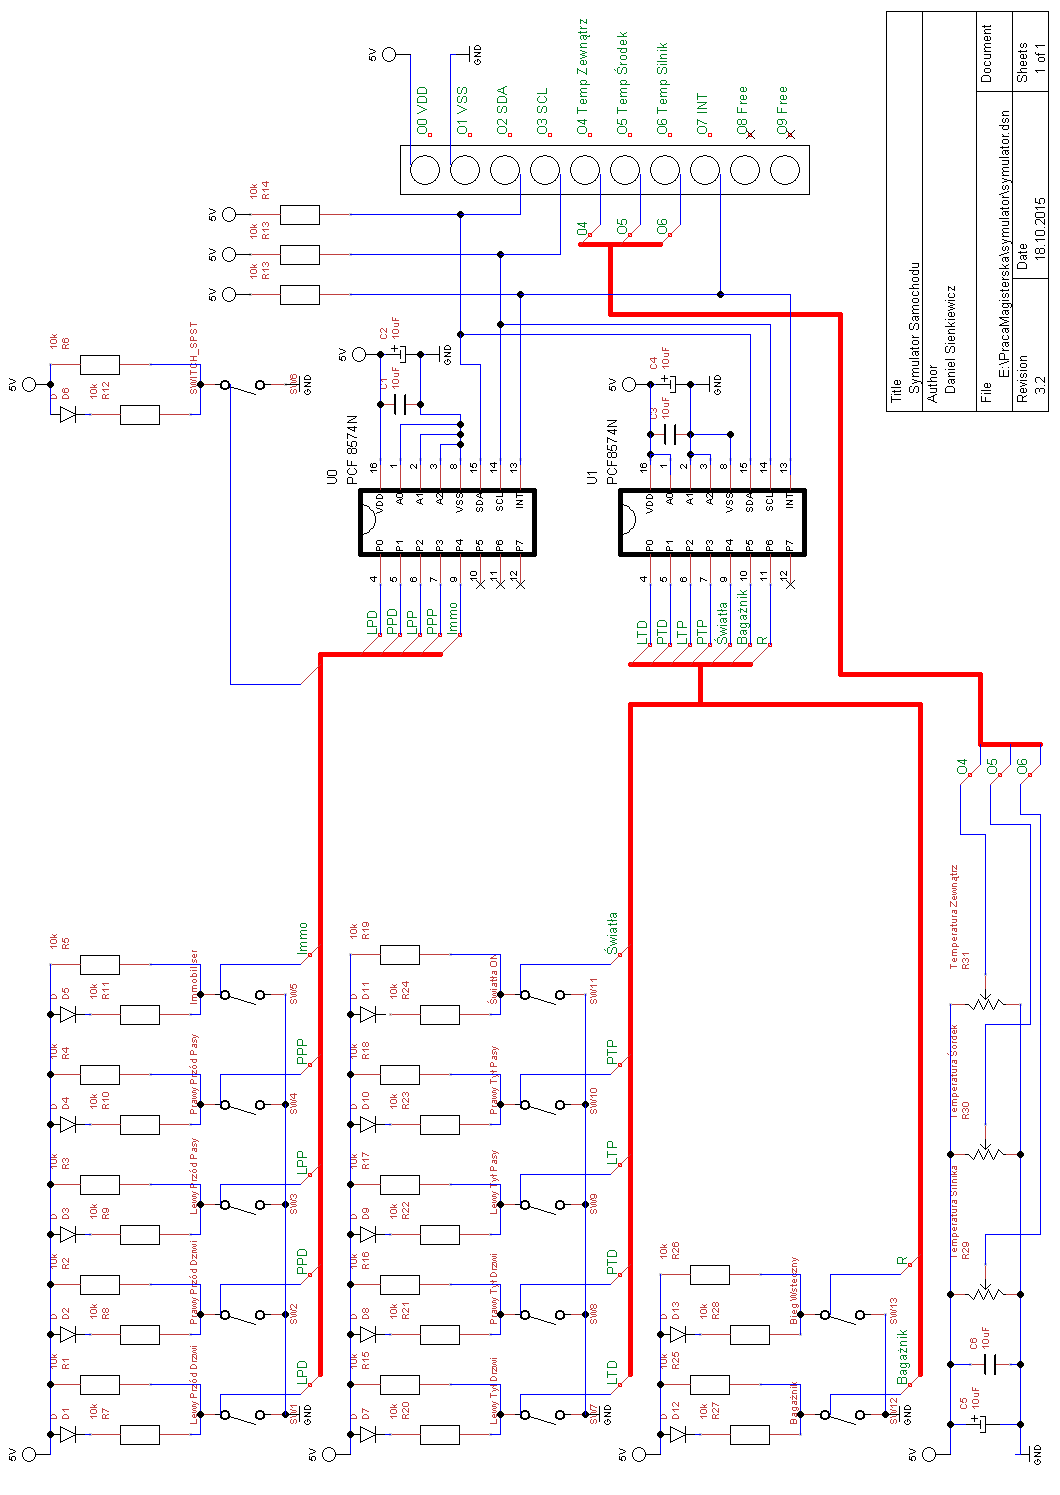
\includegraphics[height=0.4\textheight]{images/symulator.png}
    \caption{Schemat symulatora samochodu\label{SchematSymulatora}}
    \source{Opracowanie własne}
\end{figure}

\section{VM800}
  - na poczatku emulacja na PC
  - potem przepisanie na niski poziom
  - ostatecznie podpiecie do Galielo (poszukac czy juz jest?)
  
   programers manual reference vm800 ftdi POSZUKAĆ!!!!

\section{Dalsze kroki oraz propozycje}
- schemat blokowy z BAJERAMI i wybrane to co zrobię
%================KONIEC IMPLEMENTACJA=====================

\summary
TO DO

\appendix
\chapter{Karty Katalogowe}
Katalog \emph{datasheets} zawiera karty katalogowe użytych podzespołów
\chapter{Programy}
Katalogi \emph{Galileo, PCF8574N} zawierają kod źródłowy oprogramowania stworzonego na potrzeby pracy. 

\noindent Katalog \emph{Galileo} zawiera oprogramowanie mikrokomputera Intel\cite{einstein} Galileo.

\noindent Katalog \emph{PCF8574N} zawiera oprogramowanie I/O Expander PCF8574N.

\bibliographystyle{unsrt}
\bibliography{sample}

\listoftables

\listoffigures

\oswiadczenie

\end{document}